%%%%%%%%%%%%%%%%%%%%%%%%%%%%%%%%%%%%%%%%%%%%%%%%%%%%%%%%%%%%%%%%%%%%%%
%%% $LastChangedDate: 2022-04-04 16:08:53 +0200 (Mo, 04 Apr 2022) $ (local)
%%% $LastChangedRevision: 2619 $
%%% $LastChangedBy: lf1agure $
%%% $Id: usermanual.tex 2619 2022-04-04 14:08:53Z lf1agure $
%%%%%%%%%%%%%%%%%%%%%%%%%%%%%%%%%%%%%%%%%%%%%%%%%%%%%%%%%%%%%%%%%%%%%%
\documentclass[11pt,a4paper,twoside]{article}

\def\DocumentationType{User's Manual}

% Authors:
\author{%
\ProjectAdministrator\thanks{\ProjectAdministratorsFootnoteText},
%
Alexander Weber,
Elisei Macoveiciuc
}

% Abstract:
\def\AbstractText{%
\ProjectAcronym{} is a software to solve synthesis, analysis and
verification problems for infinite state dynamical systems.
%
This document provides basic information
on how to get, to compile and to use the software.
%
For more detailed information,
useful for programmers as well as for expert users,
please refer to the companion document \cite{ABS_ProgrammersManual}.
%
}

\usepackage{utils/main}

\svnid{$Id: usermanual.tex 2619 2022-04-04 14:08:53Z lf1agure $}

\usepackage{fancyvrb}

\usepackage{tikz}
\usetikzlibrary{calc,shapes,arrows,automata}


\begin{document}
\maketitle\cleardoublepage\tableofcontents\cleardoublepage

\section{Quick Start}
\label{s:QuickStart}

\ProjectAcronym{} is a software to solve synthesis, analysis and
verification problems for infinite state dynamical systems.
Follow the steps below
to quickly get a copy of \ProjectAcronym{} running on your computer,
and to see it applied to an example.

\paragraph{Prerequisites.}

\ProjectAcronym{} is an implementation
of the symbolic controller synthesis framework
introduced in \cite{ReissigWeberRungger17} and
has been presented in \cite{WeberMacoveiciucReissig22}.
Users are assumed to be familiar with both of the aforementioned
documents.
\\
\ProjectAcronym{} should be run on Linux,
which is what we assume throughout this document.
Some external software is required as well;
we recommend to proceed with the following steps and
follow the instructions printed out on the screen.
If this does not work, please refer to
\cite[Section ``System Prerequisites'']{ABS_ProgrammersManual}
for more specific requirements.

\paragraph{Obtaining a copy of \ProjectAcronym.}

\ProjectAcronym{} is maintained using the version control system
\verb|svn| \cite{svnManual11}, and access is by user
name and password.
Create a working copy of \ProjectAcronym{} in a local directory of
your choice, which may take some time:
\begin{flushleft}
\verb|>| \verb|svn checkout --username ABSpublic |
\verb|\|\\
\verb|>| \expandafter\verb\expandafter|\RootAddressOfProjectInRepository/tags/public/CurrentPublicVersion |
\verb|\|\\
\verb|>| $<$full path to working copy of \ProjectAcronym{}$>$
\end{flushleft}
%
If asked for it, you would use \verb|IuseABS| as the password.

You have only read access to \ProjectAcronym; you are not
allowed to commit to the repository hosting the software.
However, if you are a member of the project administrator's
group at the \ProjectHostInstitution, please refer to
\cite{ABS_ProgrammersManual} for other ways to get (read and write)
access.

\paragraph{License.}
\ProjectAcronym{} has been made publicly available under
GNU General Public License. For terms and conditions,
see the file \nolinkurl{trunk/COPYING}
in the working copy of \ProjectAcronym.

\paragraph{Solving a simple synthesis problem.}
Within the working copy,
navigate to the directory\linebreak{}\verb|trunk/examples/SinglePole/| and
run \verb|make|. After some time and a continuous flow of messages,
you should eventually see a message similar to the following:
\begin{verbatim}
- Results: 
  Control problem has been solved.
\end{verbatim}
%
Navigate to the directory 
\verb|trunk/examples/SinglePole/Results|
to see two output files:
%
% Version for HSCC 2022 repeatability package:
% Navigate to the directory 
% \texttt{/home/hscc2022/Documents/ABS/examples/SinglePole} 
% in the bash shell
% and run 
% \begin{verbatim}
% make 
% \end{verbatim}
% %
% After some seconds 
% you are asked to make a choice: 
% %
% Type \texttt{0} and press ENTER.
% After about a minute 
% the last message on the screen will be 
%
% \begin{verbatim}
% Results:
% Control problem has been solved.
% \end{verbatim}
% %
% Navigate to the directory 
% \texttt{/home/hscc2022/Documents/ABS/examples/SinglePole/Results}
% to see two output files:
% %
\begin{verbatim}
Controller.dat
Value_Function.dat
\end{verbatim}
%
You may modify the control problem 
in the file \texttt{SinglePole.abcs} 
(open with a text editor) and 
start all over as described above.
%
To delete all produced files, run
\begin{verbatim}
make clean
\end{verbatim}
% 
%\textcolor{red}{We need a simple example in this
%section. Requirements:
%demonstrates the formulation of a control problem, the use of
%\ProjectAcronym{} to solve the problem, as well as the use of
%produced results;
%should be part of the distribution (\nolinkurl{.../examples/});
%amenable to modification by user, who might want to
%evaluate the resulting changes in the output (in later versions,
%modification could include more complex specification such as surveilance);
%useful as a running example later on in this document, and maybe in
%the Programmer's Manual.
%Perhaps we should also present part of the theory in \cite{ReissigWeberRungger17} in
%a self-contained fashion, so that familiarity with that reference is
%an advantage but not anymore a requirement.\\
%Candidates: SinglePole; examples in manuals/papers for SCOTS, Cosyma
%}


\section{Introduction}
\label{s:intro}

\ProjectAcronym{} is an implementation
of the symbolic controller synthesis framework
introduced in \cite{ReissigWeberRungger17}.
%
The software
applies to sampled-data control systems and
to control problems with reach-avoid or invariance specification.
%
It is based on the method \cite[Th.~VIII.4]{ReissigWeberRungger17}
for computing abstractions and
the methods in
\cite{ReissigRungger19,MacoveiciucReissig18aC,MacoveiciucReissig19aC}
%\cite[Th.~IX.5]{ReissigRungger19}
for controller synthesis.
\ProjectAcronym{} is specifically described in \cite{WeberMacoveiciucReissig22}.
This manual provides more details to the input,
output and, more generally, the usage of the program.
%
%
\subsection{Processable control problems}
%
We briefly discuss the processable control problems below. 
See \ref{fig:1} for an illustration. 
The term control problem refers throughout to 
a pair of a control system (``plant") and 
a specification on that control system.

% 
The plant is a sampled-data control system 
whose underlying continuous-time dynamics
is of the form
%
\begin{equation}
\label{e:cont:dynamics}
\dot x \in f(x,u) + \segcc{-w,w},
\end{equation}
%
where $f\colon \mathbb{R}^n \times U \to \mathbb{R}^n$ 
is continuous and locally Lipschitz continuous in the first argument, 
$U \subseteq \mathbb{R}^m$ is non-empty and $w \in \mathbb{R}_+^n$. 
$x\colon \mathbb{R}_+ \to \mathbb{R}^n$ and 
$u\colon \mathbb{R}_+ \to U$ denote 
the state and input signal, respectively.
% 
%The set $W$ allows to account for uncertainties in the continuous-time dynamics. 

\ProjectAcronym{} returns static state-feedback controllers $C \colon X \rightrightarrows U$ such that 
the obtain control law takes the form
\begin{equation}
\label{e:Controller:discrete}
u(t) \in C(P(x(t))),
\end{equation}
where the map $P \colon X \rightrightarrows X$ given by $x \mapsto x + \segcc{-z,z}$ for some constant $z\in \mathbb{R}^n_+$ 
models uncertainties in the measurement of $x$.
%
%

To discuss the processable specifications, 
let $F \colon \mathbb{R}^n \times U \rightrightarrows \mathbb{R}^n$ 
denote the right hand side of the discrete-time dynamics 
obtained from sampling \ref{e:cont:dynamics} 
with a constant sampling time $\tau$ \cite[Def.~VIII.1]{ReissigWeberRungger17}. 
%
In this way, \ProjectAcronym{} actually 
works with the discrete-time dynamics
%
\begin{equation*}
x(t+1) \in F(x(t),u(t))
\end{equation*}
%
and time-discrete signals 
$x \colon \mathbb{Z}_+ \to \mathbb{R}^n$, 
$u \colon \mathbb{Z}_+ \to U$.
%	 
\subsubsection*{Reachability}
%
A reach-avoid specification asks to steer each state signal (of the sampled system) 
starting in a set $A\subseteq \mathbb{R}^n$ into 
a target set $E \subseteq \mathbb{R}^n$ in finite time 
while avoiding an obstacle set $H \subseteq \mathbb{R}^n$. 
%
More formally, the condition is
%the control problem reads: Find a controller with control law $\mu \colon \mathbb{R}^n \to U$ so that 
%\begin{equation}
%\label{e:closedloop:dynamics}
%\forall_{t \in \mathbb{Z}_+} \ x_c(t + 1) \in F\big (x_c(t),\mu(x_c(t)) \big ) 
%\end{equation}
%and 
\begin{equation}
\label{e:reach_cond}
x(t) \in A \ \Longrightarrow \ \big ( \ \exists_{T \in \mathbb{Z}_+} \ x(T) \in E \ 
\wedge \ \forall_{t \in \intcc{0;T}} \ x(t) \notin H \ \big ).
\end{equation}
%
%
and is represented by the triple $(A,H,E)$ of subsets of the state space.
%
%Here, $x_c \colon \mathbb{Z}_+ \to \mathbb{R}^n$ denotes the closed-loop state signal. 
%The controller may also have to process distorted state signals due to measurement errors.
%In this case,  in place of \ref{e:closedloop:dynamics}, dynamics
%\begin{equation}
%\label{e:closedloop:dynamics:measurementerror}
%\forall_{t \in \mathbb{Z}_+} \ x_c(t + 1) \in F\big (x_c(t),\mu(\tilde x_c(t)) \big ), 
%\end{equation}
%can be considered, where for some $z \in \mathbb{R}^n_+$ and all $t \in \mathbb{Z}_+$ we have $\tilde x_c(t) \in x_c(t) + \segcc{-z,z}$ .
%
%
\subsubsection*{Invariance}
An invariance specification asks to keep 
each state signal starting in a set $A$ indefinitely 
in a target set $E$ 
while avoiding an obstacle set $H$. 
%
To be precise, the condition is
\begin{equation}
\label{e:inv_cond}
x(0) \in A \ \Longrightarrow \ \forall_{t \in \mathbb{Z}_+} x(t) \in E \setminus H
\end{equation}
and is also represented by the triple $(A,H,E)$ of subsets of the state space.
\begin{figure}[b]
\centering
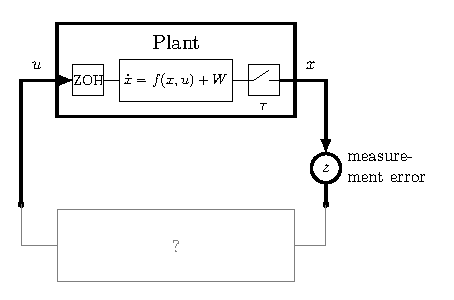
\includegraphics[scale=1]{{{figures/openloop}}}\hspace{1.0cm}
{
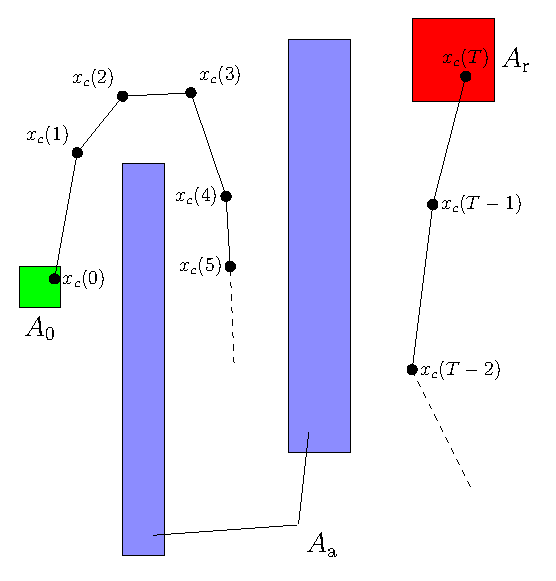
\includegraphics[scale=.6]{{{figures/reachavoid}}}
}
\caption{\label{fig:1}Illustration of the processable plant structure and a reach-avoid specification.}
\end{figure}
%
%
%
\subsection{User input and program output}
%
%
The specification of the control problem 
to solve is done by an ASCII file and 
using a special programming language (input language).
%
All the problem-specific user input (including the control problem) 
is contained in that file, which we call thereafter \concept{problem file}.

Every term written in a problem file 
is understood as a mathematical statement. 
%
That is, all the results returned from 
the software hold for the literal real numbers 
appearing in the problem file -- not for floating-point approximations of the literals.
%
For example, if the constant $\pi$
(the ratio of the circumference of a circle to the diameter) appears 
in the definition of the function $f$ in \ref{e:cont:dynamics} 
then any given result is valid for $\pi$ and 
not for some approximation of $\pi$. 
%
However, there is no guarantee that 
the software will be able to process or 
to solve the given control problem.

In the case of a successful controller synthesis 
the obtained controller is represented in an ASCII file.
% 
More precisely, the abstract controller and 
the quantizer according to \cite[Th.~VI.3]{ReissigWeberRungger17} 
are specified in that file.

\clearpage
\section{Specification of control problems}

Subsequently, the formulation of control problems and 
of other required parameters is described. 

\subsection{Preparatory actions}
%\textcolor{red}{This subsection seems to be obsolete; see \cite{ABS_ProgrammersManual}.}
%
In order to set up your own control problem the following actions must be taken:
\begin{enumerate}
\makeatletter
\def\labelenumi{\theenumi.)}
\def\theenumi{\arabic{enumi}}
\def\p@enumi#1{#1.)}
\makeatother
\item \label{a:1} Run 
\begin{verbatim}
make newproblem
\end{verbatim}
in the root directory
\item Enter a name for your new control problem
\item Enter the path to an existing directory in your system. (Do not use the tilde \verb|~| for pointing to your home directory.) In this directory, a subdirectory named as the name of your control problem will be automatically created. 
All the files related to your control problem (e.g. problem file, binary file) 
will be contained in that subdirectory. This subdirectory must not exist already
\item \label{a:3} Navigate to the previous subdirectory and open the file with file extension \texttt{abcs} using a text editor
\item Specify your control problem and other parameters in the opened file using the programming language described in the next subsection
\end{enumerate}
\begin{Example}
Taking all but the last action above the command line may look as follows
\end{Example}
\begin{verbatim}
unibw@linux:~/1.2$ make newproblem 
Please enter a name for your new control problem: Rocket
Please enter the path to an existing directory: ../ControlProblems
Specify your control problem in '../ControlProblems/Rocket/Rocket.abcs'.
unibw@linux:~/1.2$ emacs ../ControlProblems/Rocket/Rocket.abcs
\end{verbatim}

\subsection{Input language}
%\textcolor{red}{Comments: \texttt{/* ... */}}\\
We use in this section the notation of Section \ref{s:intro}.
%
We outline below the entities that the user has to specify:

%\begin{table}
\begin{center}
\begin{tabular}{lll}
Entity & Description & Type \\
\hline
\hline
$n$, $m$ & State and input space dimension & Integer \\
%$m$ & Dimension of the input space \\
$z$ & Bound for measurement 
uncertainty, cf.~\ref{e:Controller:discrete} & Vector 
\\
$\bar X_1$ & Operating range of controller & Hyper-interval
\\
$\bar U$ & Input space of right hand side of \ref{e:cont:dynamics} & Hyper-interval
\\
$f$ & Unperturbed right hand side of \ref{e:cont:dynamics}%, periods of $f$ \cite[Sec.VIII.D]{ReissigWeberRungger17} if any 
& Function 
\\
$w$ & Bound for dynamic uncertainties, cf.~\ref{e:cont:dynamics} & Vector \\
$\tau$ & Sampling time & Real number\\
\hline
$A$, $E$, $H$ & Initial, target, obstacle set, cf.~\ref{e:reach_cond}, \ref{e:inv_cond} & Union of hyper-intervals 
\\
%$E$ & Target set, as in \ref{e:reach_cond}, \ref{e:inv_cond}\\
%$H$ & Obstacle set, as in \ref{e:reach_cond}, \ref{e:inv_cond} \\
\hline
%$\eta_0$, $\eta$ & Grid parameters for abstract state space, as in \ref{e:grid} \\
%$\kappa$ & Grid parameters for abstract input space, as in \ref{e:abstract_input_space}
$d_1$, $d_2$ & State and input space discretization parameter & Vector 
\\
\hline
$p$, $q$ & Integration orders for dynamics and growth bounds & Integer
%\\
%$q$ & Integration order for approximating $\beta$ in \ref{e:abstraction:overapproximation}
\end{tabular}
\end{center}
%\caption{\label{fig:user_input_mathematically}Objects required as user input to ABS.}
%\end{table}

%\begin{center}
%\begin{tabular}{ll}
%Entity & Description \\
%\hline
%\hline
%$n$ & Dimension of the state space \\
%$m$ & Dimension of the input space \\
%$U$ & Input space of the continuous-time dynamics \\
%$f$ & As in \ref{e:cont:dynamics}, occasionally periods of $f$ \cite[Sec.VIII.D]{ReissigWeberRungger17} \\
%$w$ & Bound on the (dynamic) uncertainties, as in \ref{e:cont:dynamics} \\
%$\tau$ & Sampling time \\
%$z$ & Bound on the measurement errors, as in \ref{e:closedloop:dynamics:measurementerror} \\
%\hline
%$A_0$ & Initial set \\
%$A_\mathrm{r}$ & Target set \\
%$A_\mathrm{a}$ & Obstacle set \\
%\hline
%$\bar X_2$ & Set of compact cells for the abstraction \\
%$U_2$ & Input space of the abstraction
%\\
%\hline
% & Integration orders for numerical solutions
%\end{tabular}
%\end{center}
Subsequently, we discuss the programming language 
with which the above entities are specified. 
%
At the same time, the restrictions on the entities above due to the programming language
are explained. 
%
Thus, both the syntax and 
the semantics of the language are explained simultaneously.
%
We actually discuss only the most relevant subset
of the language. 
%
The full syntax is included in the appendix. 

Every problem file has a structure as indicated in \ref{fig:2}.
%
In the first part, auxiliary constants and hyper-intervals are defined. 
The second part contains the specification of the function $f$ in \ref{e:cont:dynamics}.
In the last part, the remaining parameters are specified. 
A comment has to be enclosed inside the strings \verb|/*| and \verb|*/|, and 
can appear anywhere in the problem file.
The file \nolinkurl{examples/SinglePole/SinglePole.abcs} is listed in \ref{fig:2}. 

We use Backus-Naur Forms for specifying the grammar, where terminals 
are printed as 
\begin{quote}
\terminal{terminal}
\end{quote}
and nonterminals as 
\begin{quote}
\nonterminal{nonterminal}
\end{quote}
Keywords (or reserved words) are printed as 
\begin{quote}
\terminalkeyword{keyword}
\end{quote}
for better readability of the forms. The two components of productions are separated by the symbol $\BNFsep$ and the alternatives in the second component are separated by a vertical bar $|$.
We refer the reader to \cite{Ginsburg66} for the concept of context-free grammars.
\begin{figure}
\begin{minipage}{.5\textwidth}
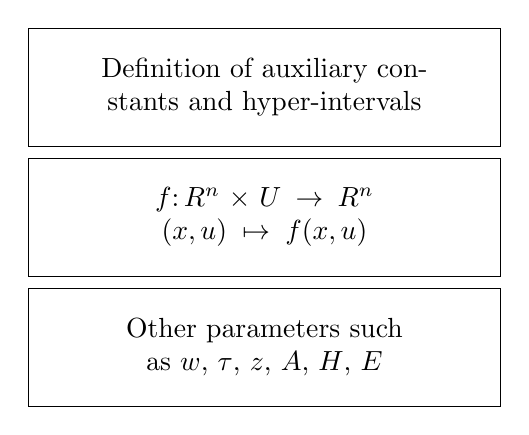
\begin{tikzpicture}[scale=1.5]
{ 
\def\offset{1.1}
\def\radius{2.}
%\node[text width=2cm,align=right] at (-\radius-.8,.5-.1) {\small \it 1st line};
\draw[] (-\radius,-.5) rectangle node[text width=5cm,align=center]{Definition of auxiliary constants and hyper-intervals} (\radius,.5);
\draw[] (-\radius,-.5-\offset) rectangle node[text width=4cm,align=center]{$f \colon \mathbb{R}^n \times U \to \mathbb{R}^n$ $(x,u) \mapsto f(x,u)$} (\radius,.5-\offset);
\draw[] (-\radius,-.5-2*\offset) rectangle node[text width=5cm,align=center]{Other parameters such as $w$, $\tau$, $z$, $A$, $H$, $E$} (\radius,.5-2*\offset);
%\node[text width=2cm,align=right] at (-\radius-.8,-.5-2*\offset+.1) {\small \it end of file};
}
\makeatletter
\let\offset\@undefined
\let\radius\@undefined
\makeatother
\end{tikzpicture}
\end{minipage}
\begin{minipage}{.5\textwidth}
\begin{Verbatim}[fontsize=\footnotesize]
Real gamma in [0.0125,0.0126]; /* Friction param. */

f: (x,u) in (Real[2],[-2,2]) to y[2]
{
 y[0] = x[1];
 y[1] = -sin(x[0])-cos(x[0])*u-2*gamma*x[1];
}

SamplingTime : 0.3;
OperatingRange: ([0,2*Pi],[-2,2]);
ListOfPeriodicComponents : (0);
InitialSet : ([0,0],[0,0]);
TargetSet : ([Pi-.1,Pi+.1],[-.1,.1]);
InitialStateSpaceSubdivision : (100,100);
InitialInputSpaceSubdivision : (3);
IntegrationOrder : 5; 
IntegrationOrderGrowthBound : 15;

/* This is a comment line */
\end{Verbatim}
\end{minipage}
\caption{\label{fig:2}problem file: Structure (l.h.s) and example (r.h.s.)}
\end{figure}
For example, we have the following productions in the grammar, 
which state, roughly speaking, 
that a digit is an Arabic numeral and an integer
is a sequence of digits.
\begin{align*}
\nonterminal{digit} &::= \terminal{0} \ | \ \terminal{1} \ | \ \terminal{2} \ | \ \terminal{3} \ | \ \terminal{4} \ | \ \terminal{5} \ | \ \terminal{6}
\ | \ \terminal{7} \ | \ \terminal{8} \ | \ \terminal{9} \\
\nonterminal{literal\_unsigned\_integer} &::= \nonterminal{digit} \ | \ \nonterminal{literal\_unsigned\_integer} \ \nonterminal{digit}
\end{align*}
\subsubsection{Constants and intervals}
A constant $c \in \mathbb{R}$ can be specified by
\begin{quote}
\terminalkeyword{Real} \nonterminal{identifier} \terminal{=} \nonterminal{expression} \terminal{;}
\end{quote}
where \nonterminal{expression} may represent an element of $\mathbb{R}$ or a term of finite compositions of the functions
\begin{center}
\begin{tabular}{ll}
$+$ & Addition \\
$-$ & Subtraction \\
$\times$ & Multiplication \\
$\div$ & Division \\
$\hat{~}$ & Exponentiation \\
$\operatorname{atan}$ & Inverse tangent \\
$\cos$ & Cosine \\
$\cosh$ & Hyperbolic cosine \\
$\exp$ & Exponential \\
$\ln$ & Natural logarithm \\
$\sin$ & Sine \\
$\sinh$ & Hyperbolic sine \\
$\operatorname{sqrt}$ & Square root \\
$\tan$ & Tangent
\end{tabular}
\end{center}
See Appendix for the full specification of \nonterminal{expression} and \nonterminal{identifier}. For example, we may write 
\begin{verbatim}
Real a = 2*Pi ; 
\end{verbatim}
for representing the circumference of the unit circle. Here, the keyword \terminalkeyword{Pi} represents $\pi$. An interval $\intcc{a,b} \subseteq \mathbb{R}$, $a\leq b$, can be specified using the production
\begin{quote}
\nonterminal{literal\_interval\_expression} ::= \terminal{[} \nonterminal{expression} \terminal{,} \nonterminal{expression} \terminal{]} \terminal{;}
\end{quote}
where \nonterminal{expression} represents $a$ and $b$ respectively.

A constant $c \in \mathbb{R}$ can also be uncertain, in which case one can use
\begin{quote}
\terminalkeyword{Real} \nonterminal{identifier} \terminalkeyword{in} \nonterminal{literal\_interval\_expression} \terminal{;}
\end{quote}
to express that $c$ is bounded in an interval but its precise value is unknown.

It is also possible to define vectors $v \in \mathbb{R}^k$ and matrices $M \in \mathbb{R}^{k \times l}$, $k,l \in \mathbb{N}$. For example, the vector $v = (\sqrt{2},2^3) \in \mathbb{R}^2$ and the matrix in $M = (\begin{smallmatrix}
1 & 2 \\ 3 & 4
\end{smallmatrix}) \in \mathbb{R}^{2\times 2}$ are represented through the lines
\begin{verbatim}
Real v[2];
v[0] = sqrt(2);
v[1] = 2^3;
\end{verbatim}
and 
\begin{verbatim}
Real M[2][2];
M[0][0] = 1;
M[0][1] = 2;
M[1][0] = 3;
M[1][1] = 4;
\end{verbatim}
respectively.
\begin{Important}
Indices of components are zero-based.
\end{Important}
\subsubsection{Hyper-intervals}
Hyper-intervals $\segcc{a,b} = \intcc{a_1,b_1} \times \ldots \times \intcc{a_n,b_n}$, $a,b \in \mathbb{R}^n$, $a\leq b$, can be specified according
\begin{quote}
\nonterminal{literal\_hyperinterval\_expression} \BNFsep \ \terminal{(} \nonterminal{interval\_expression\_list} \terminal{)} \terminal{;}
\end{quote}
where \nonterminal{interval\_expression\_list} demands the specification of the intervals $\intcc{a_i,b_i}$, $i \in \intcc{1;n}$, according \nonterminal{literal\_interval\_expression} and written in succession separated by commas. 
$\mathbb{R}^n$ itself can also be considered a hyper-interval so that hyper-intervals in total can be specified according
\begin{quote}
\nonterminal{hyperinterval\_expression} \BNFsep \ \nonterminal{literal\_hyperinterval\_expression} $|$ \terminalkeyword{Real} \terminal{[} \nonterminal{expression} \terminal{]} \terminal{;}
\end{quote}
where \nonterminal{expression} shall represent $n$.
\subsubsection{Continuous-time unperturbed dynamics}
The syntax for specifying the right hand side in \ref{e:cont:dynamics} is too complex 
to explain it using the actual productions. Therefore, we use, as it is the default in other programming books,
an example. We might write
\begin{verbatim}
f: (x,u) in (Real[2],([-2,2],[0,1])) to y[2]
{
 y[0] = x[1] ;
 y[1] = - sin(x[0]) - cos(x[0])*u[0] - u[1]*x[1] ;
}
\end{verbatim}
for representing the function $f \colon \mathbb{R}^2 \times U \to \mathbb{R}^2$ defined through
\[
f(x,u) = (x_2,-\sin(x_1)-\cos(x_1)\cdot u_1 - u_2x_2),
\] 
where $U = \intcc{-2,2} \times \intcc{0,1}$. 
%
We note that 
the identifiers \verb|x| and \verb|u| shall function in every problem file
as the state and input variable. So, \verb|x| and \verb|u| are keywords of the input language.
%
The dimension $n$ shall appear to the right of the image variable (in the example code it is \verb|y|)
and the dimension $m$ is implicitly specified through the hyper-interval that is associated to \verb|u|. 
\begin{Important}
The input space $U$ is also been defined through the previous code fragment. 
$U$ shall be a compact hyper-interval.
\end{Important}
\begin{Important}
Indices of components are zero-based.
\end{Important}
\subsubsection{Bound on dynamic uncertainties}
The bound on the dynamic uncertainties $w$ is specified according 
\begin{quote}
\terminalkeyword{BoundOnDynamicUncertainties} \ \terminal{:} \ \nonterminal{expression\_tuple} \terminal{;}
\end{quote}
where \nonterminal{expression\_tuple} represents an $n$-tuple of non-negative real numbers. For example, 
\begin{verbatim}
BoundOnDynamicUncertainties : (0,1/2) ; 
\end{verbatim}
represents $w = (0,\frac{1}{2}) \in \mathbb{R}^2$. \\
This specification shall appear at most once in the problem file. 
Non-appearance means $w = 0$. 
\subsubsection{Sampling time}
The sampling time $\tau$ is specified according 
\begin{quote}
\terminalkeyword{SamplingTime} \ \terminal{:} \ \nonterminal{literal\_unsigned\_number} \terminal{;}
\end{quote}
where \nonterminal{literal\_unsigned\_number} shall be a positive real number.\\
This specification shall appear exactly once in the problem file. 
\subsubsection{Bound on measurement errors}
The bound $z$ on the measurement errors is specified according 
\begin{quote}
\terminalkeyword{BoundOnMeasurementErrors} \ \terminal{:} \ \nonterminal{expression\_tuple} \terminal{;}
\end{quote}
where \nonterminal{expression\_tuple} represents an $n$-tuple of non-negative real numbers. \\
This specification shall appear at most once in the problem file. 
Non-appearance means $z = 0$.
%
\subsubsection{Specifications}
The triple $(A,H,E)$ representing both a reachability problem and an invariance problem is specified as follows. 
Each of the sets $A$, $H$, $E$ may be a 
finite union of compact hyper-intervals in $\mathbb{R}^n$, where every member of the union is specified according to the respective rules below. 
If $k$ lines according to such a rule appear appropriately in the problem file then the set is a union of $k$ (not necessarily distinct) hyper-intervals.
\begin{itemize}
\item $A$:
\begin{quote}
\terminalkeyword{InitialSet} \ \terminal{:} \ \nonterminal{literal\_hyperinterval\_expression} \terminal{;}
\end{quote}
This specification shall appear at least once. 
\item $E$:
\begin{quote}
\terminalkeyword{TargetSet} \ \terminal{:} \ \nonterminal{literal\_hyperinterval\_expression} \terminal{;}
\end{quote}
This specification shall appear at least once. 
\item $H$:
\begin{quote}
\terminalkeyword{ObstacleSet} \ \terminal{:} \ \nonterminal{literal\_hyperinterval\_expression} \terminal{;}
\end{quote}
Non-appearance of this specification means $H = \emptyset$.
\end{itemize}
\subsubsection{Abstraction}
\begin{itemize}
\item
The (finite) set $\bar X_2$ is specified implicitly by specifying 
\begin{itemize}
\item a hyper-interval $\segcc{a,b}$, $a,b \in \mathbb{R}^n$, $a < b$ according

\begin{quote}
\terminalkeyword{OperatingRange} \ \terminal{:} \ \nonterminal{literal\_hyperinterval\_expression} \terminal{;}
\end{quote}
This specification shall appear exactly once.
\item an integer vector $p \in \mathbb{N}^n$ according 
\begin{quote}
\terminalkeyword{InitialStateSpaceSubdivision} \ \terminal{:} \ \nonterminal{literal\_unsigned\_integer\_tuple} \terminal{;}
\end{quote}
This specification shall appear exactly once.
\end{itemize}
%
The hyper-interval $\segcc{a,b} = \intcc{a_1,b_1} \times \ldots \times \intcc{a_n,b_n}$ is 
the set $\cup_{x_2 \in \bar X_2} x_2$ 
and so $\bar X_2$ is implicitly defined by subdividing every edge $\intcc{a_i,b_i}$ of $\segcc{a,b}$ into $d_{1,i}$ intervals of equal length. 
%
More concretely, $x_2 \in \bar X_2$ if and only if there exists $k \in \mathbb{Z}^n_+$ satisfying $k_i \in \intcc{0;d_{1,i}-1}$ for every $i \in \intcc{1;n}$ and
\begin{equation*}
x_2 = a + v(k) + \segcc{0,\eta},
\end{equation*}
where $v(k)_i \defas k_i \eta_i$, $\eta_i = (b_i-a_i)/d_{1,i}$, $i \in \intcc{1;n}$. 

If there exists a subset $I \subseteq \intcc{1;n}$ so that $f$ possesses the property
\begin{equation}
\label{e:periods}
f(x + (b_i - a_i)e_i ) = f(x)
\end{equation}
for every $x \in \mathbb{R}^n$ and $i \in I$ then one may include a line according
\begin{quote}
\terminalkeyword{ListOfPeriodicComponents} \ \terminal{:} \ \nonterminal{literal\_unsigned\_integer\_tuple} \terminal{;}
\end{quote}
to represent that property. In \ref{e:periods}, $e_i$ denotes the $i$th standard basis vector of $\mathbb{R}^n$.
\begin{Note} The indices have to be specified zero-based. \end{Note}
\item The (finite) set $U_2$ is specified implicitly by specifying an integer vector $p' \in \mathbb{N}^m$ according
\begin{quote}
\terminalkeyword{InitialInputSpaceSubdivision} \ \terminal{:} \ \nonterminal{literal\_unsigned\_integer\_tuple} \terminal{;}
\end{quote}

The set $U_2$ is then obtained by subdividing the $i$th edge of $U$ into $d_{2,i}$ intervals of equal length, $i \in \intcc{1;m}$.
%
More concretely, $u_2 \in \bar U_2$ if and only if there exists $k \in \mathbb{Z}^m_+$ satisfying $k_i \in \intcc{0;d_{2,i}-1}$ for every $i \in \intcc{1;m}$ and
\begin{equation*}
u_2 = a' + v(k) + \eta'/2,
\end{equation*}
where $v(k)_i \defas k_i \eta'_i$, $\eta'_i = (b'_i-a'_i)/d_{2,i}$, $i \in \intcc{1;m}$, $U = \segcc{a',b'}$, $a' \leq b'$. 
\end{itemize}
\subsubsection{Order of integrations}
The method \cite[Th.~VIII.4]{ReissigWeberRungger17} involves the general solution of the unperturbed dynamics $\dot x = f(x,u)$. 
However, the general solution is usually not available as an explicit formula. Therefore, the 
implementation uses a Taylor polynomial as an approximation formula instead. 
In the current version, the degree of the polynomial (order of the approximation formula)
has to be specified by the user. This is done according
\begin{quote}
\terminalkeyword{IntegrationOrder} \ \terminal{:} \ \nonterminal{literal\_unsigned\_integer} \terminal{;}
\end{quote}
where the integer shall be positive. Accordingly, 
\begin{quote}
\terminalkeyword{IntegrationOrderGrowthBound} \ \terminal{:} \ \nonterminal{literal\_unsigned\_integer} \terminal{;}
\end{quote}
specifies the degree of the polynomial used to 
approximate the growth bound formula.
\section{Controller synthesis}
\subsection{Starting the computation}
Having specified the control problem and the other parameters the command 
\begin{verbatim}
make 
\end{verbatim}
run in the problem directory will successively run
\begin{enumerate}
\makeatletter
\def\labelenumi{\theenumi.)}
\def\theenumi{\arabic{enumi}}
\def\p@enumi#1{#1.)}
\makeatother
\item the generation of problem-dependent \textbf{source code}
\item the compilation of a binary file for the controller synthesis for this control \textbf{system}
\item the \textbf{controller} synthesis
\end{enumerate}
Usually, it is more convenient to launch the previous steps manually. (For example, when performing the first and second step on a laptop but the computationally most expensive last step on a remote workstation.)
The following commands are provided for this purpose:
\begin{enumerate}
\makeatletter
\def\labelenumi{\theenumi.)}
\def\theenumi{\arabic{enumi}}
\def\p@enumi#1{#1.)}
\makeatother
\item \verb|make sourcecode|
\item \verb|make system|
\item \verb|make controller|
\end{enumerate}
\begin{Note} After \verb|make controller| the user is asked to choose the actual algorithm to be applied. After that the actual computation starts. See Section \ref{ss:userchoices}.
\end{Note}
Additionally, the command \verb|make clean| will remove all files and directories that have been automatically generated by \ProjectAcronym. The problem file will not be removed.

\subsection{User choices}
In the current version, the user has the following choices:
\begin{itemize}
\item[0.] On-the-fly solution to the reach avoid problem. Algorithms as in \cite{MacoveiciucReissig18aC}.
\item[1.] On-the-fly solution to the invariance  problem.  Algorithms as in \cite{MacoveiciucReissig19aC}.

(!) Note that this option currently assumes that
the set indicated as "OperatingRange" in the input file
contains apriori enclosure of the forwards reachable set of the set indicated as "TargetSet". If this is not known, option 4. would assist the user to formulate the problem correctly following the steps:
\begin{itemize}
	\item[i.] Construct an input file with the same problem data
	except for replacing numerical values to the right  of "OperatingRange" with numerical values to the right of "TargetSet".
	\item[ii.] Run  \verb|make| and choose 'Compute apriori enclosure and quit'
	\item [iii.]Compare the set  in the output (denoted here by $A$ ) with the set  introduced as "OperatingRange" in the original input file (denoted here by $B$ ).
	\item[iv.] If $A\subseteq B$ then do not change anything in
	the original input file. Go to vi.
	\item[v.] If $B\setminus A\neq \emptyset$ then in the original input file replace numerical values to the right  of "OperatingRange" (set $B$) with numerical values of the set $B \cup A$. Go to vi.
	\item[vi.] Run  \verb|make| , choose option 1.
\end{itemize}
\item[2.] Standard solution to the reach avoid problem. See \cite{MacoveiciucReissig18aC,ReissigWeberRungger17}.
\item[3.] Standard solution to the invariance  problem. See \cite{MacoveiciucReissig19aC}.
\item[4.] Compute apriori enclosure and quit. This auxiliary function output an apriori enclosure of the forward reachable set of the operating range. It may be useful to formulate invariance problems.
\end{itemize}
\label{ss:userchoices}

\subsection{Output files}

In the case of a successful controller synthesis the file
\verb|Controller.dat| will be created in the directory \verb|Results|,
where the latter is a subdirectory of the directory where the control
problem has been specified. The file structure is as below.

\begin{center}
\renewcommand{\arraystretch}{1.1}%
\tabcolsep0pt
\begin{tabularx}{\linewidth}{lp{5pt}|p{5pt}X}
line $i$ &&& Content \\
\hline
\hline
$i=1$ &&& $n$ \\
$i=2$ &&& $m$ \\
$i=3$ &&& operating range \\
$i=4$ &&& $U$ \\
\hline
$i=5$ &&& state space discretization \\
\hline
$i=6$ &&& input space discretization \\
\hline
$i=7$ &&& Information on encoding for line $9$ on \\
$i=8$ &&& Information on encoding for line $9$ on  \\
\hline
$i \in \intcc{o;o+|\bar X_2|-1}$, &&& Index of the control symbol for the cell with index $k$,
\\
where $o=9$ &&&  where $i=o+k$ is the corresponding line. \\ 
&&& A dash \verb|-| indicates that the value function is either $0$ or $\infty$ on the cell.
\end{tabularx}
\end{center}

\cleardoublepage
\appendix
\section*{Appendix}
\addcontentsline{toc}{section}{Appendix}

For the understanding of the input language, the user should be
familiar with context-free grammars and Backus-Naur forms
\cite{Ginsburg66} in the way those concepts are utilized for defining
the syntax of programming languages. For example, the grammars for the
C and Ada programming languages are included in
\cite{KernighanRitchie88} and \cite{Barnes14}, respectively.
%
In the context of control theory, we remark that in
\cite{MouelhiGirardGossler13,MouelhiGirardGoessler12} the input language used therein is also
defined using a context-free grammar.

It is important to note that the grammar is much larger than required for a problem file. 
The reason is that the grammar is also internally used for other purposes such as rounding error estimations. 
We want the grammar printed in this manual to coincide with the grammar in the implementation.
%\textcolor{red}{Does this grammar describe the language that is
%  actually available to the user?}

\section*{Grammar}
\label{s:grammar}
\subsubsection*{Start symbol (Input file structure)}
\begin{align*}
\nonterminal{program}		        
	\BNFsep \ & \nonterminal{function\_definition}                   \\                              
	| \ & \nonterminal{function\_definition} \ \nonterminal{parameter\_list}       \\                              
	| \ & \nonterminal{function\_definition} \ \nonterminal{ode\_definition}         \\                         
	| \ & \nonterminal{statement\_list} \ \nonterminal{function\_definition}                    \\              
	| \ & \nonterminal{statement\_list} \ \nonterminal{function\_definition} \ \nonterminal{parameter\_list}      \\                
	| \ & \nonterminal{statement\_list} \ \nonterminal{function\_definition} \ \nonterminal{ode\_definition}      \\  
\end{align*}
\subsubsection*{Statements}
\begin{align*}
\nonterminal{statement}  
	\BNFsep \ & \nonterminal{declaration} \\               
	| \ & \nonterminal{definition}   \\              
	| \ & \nonterminal{declaration\_and\_definition} \\
	| \ & \nonterminal{iteration\_statement}    \\  
 \nonterminal{declaration} 	
	\BNFsep \ & \terminalkeyword{Real} \ \nonterminal{component\_expression} \ \terminal{;} \\
	| \ &\terminalkeyword{Interval} \ \nonterminal{component\_expression} \ \terminal{;} \\
	\nonterminal{definition}  
	\BNFsep \ & \nonterminal{component\_expression} \ \terminal{=} \  \nonterminal{expression}  \ \terminal{;} \\
    | \ & \nonterminal{component\_expression} \ \terminal{=} \  \nonterminal{literal\_interval\_expression} \ \terminal{;} \\
	| \ & \nonterminal{component\_expression} \  \terminalkeyword{in} \ \nonterminal{interval\_expression} \ \terminal{;} \\
	\nonterminal{declaration\_and\_definition} 
	\BNFsep  \ & \terminalkeyword{Real}  \    \nonterminal{identifier} \ \terminal{=} \  \nonterminal{expression}          \ \terminal{;} \\
	|  \ & \terminalkeyword{Interval} \ \nonterminal{identifier} \ \terminal{=} \  \nonterminal{literal\_interval\_expression} \ \terminal{;} \\ 
	| \ & \terminalkeyword{Real}   \   \nonterminal{identifier}  \  \terminalkeyword{in} \ \nonterminal{literal\_interval\_expression} \ \terminal{;} \\  
\end{align*}
\begin{align*}
\nonterminal{compound\_statement }
\BNFsep \ & \terminal{\{} \ \nonterminal{statement\_list} \ \terminal{\}} \\
\nonterminal{iteration\_head} 
	\BNFsep  \ &  \terminalkeyword{for} \ \terminal{(} \nonterminal{identifier} \terminal{=} \nonterminal{expression} \terminal{,} \nonterminal{expression}  \terminal{,}  \terminal{+} \terminal{)}        \\
	| \ & \terminalkeyword{for} \ \terminal{(} \nonterminal{identifier} \terminal{=} \nonterminal{expression} \terminal{,} \nonterminal{expression} \terminal{,}  \terminal{-} \terminal{)}             \\   
\nonterminal{iteration\_statement}
	\BNFsep \ & \nonterminal{iteration\_head} \ \nonterminal{compound\_statement}       \\            
	\nonterminal{statement\_list}
\BNFsep \ &\nonterminal{statement}           \\        
| \ & \nonterminal{statement\_list} \ \nonterminal{statement}  \\ 
\end{align*}
\subsubsection*{Identifiers and literal nonnegative numbers}
\begin{align*}
  \nonterminal{identifier}
 	\BNFsep \ & \nonterminal{nondigit} \\
 	| \ & \nonterminal{identifier} \ \nonterminal{nondigit} \\
 	| \ & \nonterminal{identifier} \ \nonterminal{digit} \\
\nonterminal{literal\_unsigned\_integer} \BNFsep  \ & \nonterminal{digit} \ | \ \nonterminal{literal\_unsigned\_integer} \ \nonterminal{digit} \\
\nonterminal{digit}  \BNFsep \ & \terminal{0} \ | \ \terminal{1} \ | \ \terminal{2} \ | \ \terminal{3} \ | \ \terminal{4} \ | \ \terminal{5} \ | \ \terminal{6}
\ | \ \terminal{7} \ | \ \terminal{8} \ | \ \terminal{9} \\
\nonterminal{nondigit} \BNFsep \ & \terminal{a} \ | \ \terminal{b} \ | \ \terminal{c} \ | \ \terminal{d} \ | \ \terminal{e} \ | \ \terminal{f} \ | \ \terminal{g} \ | \ \terminal{h} \ | \ \terminal{i} \ | \ \terminal{j} \ | \ \terminal{k} \ | \ \terminal{l} 
 	\ | \ \terminal{m} \\  | \ & \terminal{n} \ | \ \terminal{o} \ | \ \terminal{p} \ | \ \terminal{q} \ | \ \terminal{r} \ | \ \terminal{s} \ | \ \terminal{t} \ | \ \terminal{u} \ | \ \terminal{v} \ | \ \terminal{w} \ | \ \terminal{x} 
 	\ | \ \terminal{y} \ | \ \terminal{z} \\ | \ & \terminal{A} \ | \ \terminal{B} \ | \ \terminal{C} \ | \ \terminal{D} \ | \ \terminal{E} \ | \ \terminal{F} \ | \ \terminal{G} \ | \ \terminal{H} \ | \ \terminal{I} \ | \ \terminal{J} 
 	\ | \ \terminal{K} \ | \ \terminal{L} \ | \ \terminal{M} \\ | \ & \terminal{N} \ | \ \terminal{O} \ | \ \terminal{P} \ | \ \terminal{Q} \ | \ \terminal{R} \ | \ \terminal{S} \ | \ \terminal{T} \ | \ \terminal{U} \ | \ \terminal{V}
 	\ | \ \terminal{W} \ | \ \terminal{X} \ | \ \terminal{Y} \ | \ \terminal{Z} \ | \ \terminal{\_} 
\end{align*}
\begin{align*}
   \nonterminal{literal\_unsigned\_decimal}
 	\BNFsep \ & \nonterminal{literal\_unsigned\_integer} \ \terminal{.} \ \nonterminal{literal\_unsigned\_integer} 
 	\\ | \ & \ \terminal{.} \ \nonterminal{literal\_unsigned\_integer}
\\ | \ & \nonterminal{literal\_unsigned\_integer} \ \terminal{.} \
 	\\ | \ & \nonterminal{literal\_unsigned\_integer} \ \terminal{.} \ \nonterminal{literal\_unsigned\_integer} \ \terminal{E} \ \ \terminal{+} \ \nonterminal{literal\_unsigned\_integer}
 	\\ | \ & \nonterminal{literal\_unsigned\_integer} \ \terminal{.} \ \nonterminal{literal\_unsigned\_integer} \ \terminal{E} \ \ \terminal{-} \ \nonterminal{literal\_unsigned\_integer}
 	\\ | \ & \nonterminal{literal\_unsigned\_integer} \ \terminal{.} \ \ \terminal{E} \ \ \terminal{+} \ \nonterminal{literal\_unsigned\_integer}
 	\\ | \ & \nonterminal{literal\_unsigned\_integer} \ \terminal{.} \ \ \terminal{E} \ \ \terminal{-} \ \nonterminal{literal\_unsigned\_integer}
 	\\ | \ & \ \terminal{.} \ \nonterminal{literal\_unsigned\_integer} \ \terminal{E} \ \ \terminal{+} \ \nonterminal{literal\_unsigned\_integer}
 	\\ | \ & \ \terminal{.} \ \nonterminal{literal\_unsigned\_integer} \ \terminal{E} \ \ \terminal{-} \ \nonterminal{literal\_unsigned\_integer}
 	\\ | \ & \nonterminal{literal\_unsigned\_integer} \ \terminal{.} \ \nonterminal{literal\_unsigned\_integer} \ \terminal{e} \ \ \terminal{+} \ \nonterminal{literal\_unsigned\_integer}
 	\\ | \ & \nonterminal{literal\_unsigned\_integer} \ \terminal{.} \ \nonterminal{literal\_unsigned\_integer} \ \terminal{e} \ \ \terminal{-} \ \nonterminal{literal\_unsigned\_integer}
 	\\ | \ & \nonterminal{literal\_unsigned\_integer} \ \terminal{.} \ \ \terminal{e} \ \ \terminal{+} \ \nonterminal{literal\_unsigned\_integer}
 	\\ | \ & \nonterminal{literal\_unsigned\_integer} \ \terminal{.} \ \ \terminal{e} \ \ \terminal{-} \ \nonterminal{literal\_unsigned\_integer}
 	\\ | \ & \ \terminal{.} \ \nonterminal{literal\_unsigned\_integer} \ \terminal{e} \ \ \terminal{+} \ \nonterminal{literal\_unsigned\_integer}
 	\\ | \ & \ \terminal{.} \ \nonterminal{literal\_unsigned\_integer} \ \terminal{e} \ \ \terminal{-} \ \nonterminal{literal\_unsigned\_integer}
 	\\ | \ & \nonterminal{literal\_unsigned\_integer} \ \terminal{.} \ \nonterminal{literal\_unsigned\_integer} \ \terminal{E} \ \nonterminal{literal\_unsigned\_integer}
 	\\ | \ & \nonterminal{literal\_unsigned\_integer} \ \terminal{.} \ \ \terminal{E} \ \nonterminal{literal\_unsigned\_integer}
 	\\ | \ & \ \terminal{.} \ \nonterminal{literal\_unsigned\_integer} \ \terminal{E} \ \nonterminal{literal\_unsigned\_integer}
 	\\ | \ & \nonterminal{literal\_unsigned\_integer} \ \terminal{.} \ \nonterminal{literal\_unsigned\_integer} \ \terminal{e} \ \nonterminal{literal\_unsigned\_integer}
 	\\ | \ & \nonterminal{literal\_unsigned\_integer} \ \terminal{.} \ \ \terminal{e} \ \nonterminal{literal\_unsigned\_integer}
 	\\ | \ & \ \terminal{.} \ \nonterminal{literal\_unsigned\_integer} \ \terminal{e} \ \nonterminal{literal\_unsigned\_integer}
\end{align*}
\subsubsection*{Expressions}
\begin{align*}
\nonterminal{component\_expression} \BNFsep 
    \ &\nonterminal{identifier} \\ 
   | \ &\nonterminal{identifier} \ \terminal{[} \ \nonterminal{expression} \ \terminal{]} \\
   | \ &\nonterminal{identifier} \ \terminal{[} \ \nonterminal{expression} \ \terminal{]} \terminal{[} \ \nonterminal{expression} \ \terminal{]} \\
\nonterminal{expression} \BNFsep 
	  \ &\nonterminal{multiplicative\_expression} \\
	| \ &\nonterminal{expression}\ \terminal{+} \ \nonterminal{multiplicative\_expression}     \\
	| \ &\nonterminal{expression}\ \terminal{-} \ \nonterminal{multiplicative\_expression}     \\
\nonterminal{multiplicative\_expression} \BNFsep 
	\ &\nonterminal{signed\_expression} \\
	| \ &\nonterminal{multiplicative\_expression} \ \terminal{*} \ \nonterminal{signed\_expression} \\
	| \ &\nonterminal{multiplicative\_expression} \ \terminal{/}  \ \nonterminal{signed\_expression} \\
\nonterminal{signed\_expression} \BNFsep
	\ &\nonterminal{exponential\_expression} \\
	| \ &\terminal{-} \ \nonterminal{exponential\_expression} \\
	| \ &\terminal{+} \ \nonterminal{exponential\_expression}  \\
\nonterminal{exponential\_expression} \BNFsep 
	\ &\nonterminal{primary\_expression} \\
	| \ &\nonterminal{primary\_expression} \ \terminal{\char94} \ \nonterminal{signed\_expression} \\
\nonterminal{primary\_expression} \BNFsep
	\ &\nonterminal{component\_expression} \\
     | \ &\nonterminal{literal\_unsigned\_number} \\
	| \ &\nonterminal{elementary\_function\_expression} \\					
	| \ &\terminal{(} \ \nonterminal{expression} \ \terminal{)}\\
\nonterminal{elementary\_function\_expression} \BNFsep
	\ &\nonterminal{name\_of\_elementary\_function} \terminal{(} \ \nonterminal{expression} \ \terminal{)} \\
\nonterminal{name\_of\_elementary\_function} \BNFsep \ &\terminalkeyword{atan} \ | \ \terminalkeyword{cos} \ | \ \terminalkeyword{cosh} \ | \
\terminalkeyword{exp} \ | \ \terminalkeyword{ln} \ | \ \terminalkeyword{sin} \ | \ \terminalkeyword{sinh} \ | \ \terminalkeyword{sqrt} \ | \
\terminalkeyword{tan} \\
\nonterminal{literal\_unsigned\_number} \BNFsep 
	\ & \nonterminal{literal\_unsigned\_integer} \\
	| \ &\nonterminal{literal\_unsigned\_decimal} \\
	| \ &\terminalkeyword{Pi} 
\end{align*}
\subsubsection*{Identifier and component expression lists}
\begin{align*}
\nonterminal{identifier\_list}
	\BNFsep \ & \nonterminal{identifier}  \\                      
	| \ & \nonterminal{identifier\_list} \  \terminal{,} \ \nonterminal{identifier}    \\
\nonterminal{identifier\_tuple}
	\BNFsep \ & \terminal{(} \ \nonterminal{identifier\_list} \ \terminal{)}      \\     
\nonterminal{component\_expression\_list}  
	\BNFsep \ & \nonterminal{component\_expression}          \\                          
	| \ & \nonterminal{component\_expression\_list} \ \terminal{,} \ \nonterminal{component\_expression}   \\    
\nonterminal{component\_expression\_tuple}  
	\BNFsep \ & \terminal{(} \ \nonterminal{component\_expression\_list} \ \terminal{)} \\  
\end{align*}
\subsubsection*{Intervals}
\begin{align*}
\nonterminal{literal\_interval\_expression}
	\BNFsep \ & \terminal{[} \ \nonterminal{expression}  \ \terminal{,} \ \nonterminal{expression} \ \terminal{]} \\
\nonterminal{interval\_expression}
	\BNFsep \ & \nonterminal{component\_expression}                      \\
	| \ & \nonterminal{literal\_interval\_expression}     \\
	| \ & \terminalkeyword{Real}					\\
\nonterminal{interval\_expression\_list}
	\BNFsep \ & \nonterminal{interval\_expression}                                   \\
	| \ & \nonterminal{interval\_expression\_list} \ \terminal{,} \ \nonterminal{interval\_expression}    \\  
\end{align*}
\subsubsection*{Hyper-intervals}
\begin{align*}
\nonterminal{literal\_hyperinterval\_expression} 
	\BNFsep \ & \terminal{(} \ \nonterminal{interval\_expression\_list} \ \terminal{)}  \\
\nonterminal{hyperinterval\_expression}
	\BNFsep \ & \nonterminal{literal\_hyperinterval\_expression}  \\
	| \ & \terminalkeyword{Real} \ \terminal{[} \ \nonterminal{expression} \ \terminal{]}         \\   
\nonterminal{interval\_hyperinterval\_expression\_list}
	\BNFsep \ & \nonterminal{interval\_expression}               \\                                    
	| \ & \nonterminal{hyperinterval\_expression}            \\                                  
	| \ & \nonterminal{interval\_hyperinterval\_expression\_list} \  \terminal{,} \ \nonterminal{interval\_expression}          \\
	| \ & \nonterminal{interval\_hyperinterval\_expression\_list} \  \terminal{,} \ \nonterminal{hyperinterval\_expression}     \\
\nonterminal{interval\_hyperinterval\_expression\_tuple}
	\BNFsep \ & \terminal{(} \ \nonterminal{interval\_hyperinterval\_expression\_list} \ \terminal{)} \\
	\end{align*}
\subsubsection*{Explicitly defined function}
	\begin{align*}
\nonterminal{function\_definition}
	\BNFsep \ &  \nonterminal{function\_declaration} \ \nonterminal{function\_head} \ \nonterminal{compound\_statement} \\
\nonterminal{function\_declaration} 
	\BNFsep \ & \nonterminal{identifier} \terminal{:}                  \\
\nonterminal{function\_image} \BNFsep \ & \nonterminal{component\_expression\_tuple} \\
	| \ & \nonterminal{component\_expression} \\
\nonterminal{function\_head} \BNFsep \ & \nonterminal{identifier} \ \terminalkeyword{in} \  \nonterminal{interval\_expression} \ \terminalkeyword{to} \ \nonterminal{function\_image}   \\
	| \ & \nonterminal{identifier}     \   \terminalkeyword{in}  \ \nonterminal{hyperinterval\_expression} \ \terminalkeyword{to} \ \nonterminal{function\_image}\\
	| \ & \nonterminal{identifier\_tuple} \  \terminalkeyword{in}  \ \nonterminal{interval\_hyperinterval\_expression\_tuple} \ \terminalkeyword{to} \ \nonterminal{function\_image} \\
		\end{align*}
\subsubsection*{Ordinary differential equation}
		\begin{align*}
\nonterminal{ode\_definition}
	\BNFsep \ & \nonterminal{function\_declaration} \ \nonterminal{function\_head \nonterminal} \ \nonterminal{ode\_statement}          \\
	\nonterminal{ode\_statement}
	\BNFsep \ & \terminal{\{} \ \nonterminal{ode\_equation} \ \terminal{;} \ \nonterminal{initialvalue\_list} \ \terminal{\}} \\
	| \ & \terminal{\{}  \ \nonterminal{initialvalue\_list} \ \nonterminal{ode\_equation} \ \terminal{;} \ \terminal{\}} \\ 
		\nonterminal{ode\_equation}
	\BNFsep \ & \terminalkeyword{diff} \ \terminal{(} \ \nonterminal{identifier}   \     \terminal{,} \ \nonterminal{identifier} \ \terminal{)} \ \terminal{=}  \ \nonterminal{identifier} \ \nonterminal{identifier\_tuple} \\
	| \ & \terminalkeyword{diff} \ \terminal{(} \ \nonterminal{identifier\_tuple} \ \terminal{,} \ \nonterminal{identifier} \  \terminal{)} \ \terminal{=} \ \nonterminal{identifier} \ \nonterminal{identifier\_tuple} \\
\nonterminal{initialvalue}
	\BNFsep \ & \terminalkeyword{initialvalue} \ \terminal{(} \ \nonterminal{component\_expression} \ \terminal{,}  \ \nonterminal{expression} \  \terminal{)} \ \terminal{;} \\
\nonterminal{initialvalue\_list }
	\BNFsep \ & \nonterminal{initialvalue}                            \\
	| \ & \nonterminal{initialvalue\_list} \ \nonterminal{initialvalue}         \\
\end{align*}
\subsubsection*{Parameters}
\begin{align*}
\nonterminal{literal\_unsigned\_integer\_list}
	\BNFsep \ & \nonterminal{literal\_unsigned\_integer} \\                                      
	| \ & \nonterminal{literal\_unsigned\_integer\_list} \ \terminal{,} \ \nonterminal{literal\_unsigned\_integer}    \\
\nonterminal{literal\_unsigned\_integer\_tuple}
	\BNFsep \ & \terminal{(} \ \nonterminal{literal\_unsigned\_integer\_list} \ \terminal{)}     \\               
\nonterminal{expression\_list}
	\BNFsep \ & \nonterminal{expression}   \\                                
	| \ & \nonterminal{expression\_list} \ \terminal{,} \ \nonterminal{expression}           \\   
\nonterminal{expression\_tuple}
	\BNFsep \ & \terminal{(} \  \nonterminal{expression\_list} \ \terminal{)}        \\       
\nonterminal{parameter\_list}
	\BNFsep \ & \nonterminal{parameter}       \\                   
	| \ & \nonterminal{parameter\_list} \ \nonterminal{parameter}      	\\
\nonterminal{parameter}
	\BNFsep \ & \terminalkeyword{ListOfPeriodicComponents}      \       \terminal{:}  \ \nonterminal{literal\_unsigned\_integer\_tuple}  \ \terminal{;} \\
     | \ & \terminalkeyword{InitialStateSpaceSubdivision}  \ \terminal{:} \ \nonterminal{literal\_unsigned\_integer\_tuple} \  \terminal{;} \\
    | \ & \terminalkeyword{InitialInputSpaceSubdivision}  \ \terminal{:} \ \nonterminal{literal\_unsigned\_integer\_tuple} \  \terminal{;} \\
	| \ & \terminalkeyword{SamplingTime}     \   \terminal{:} \ \nonterminal{literal\_unsigned\_number}           \         \terminal{;} \\
     | \ & \terminalkeyword{InitialSet}      \    \terminal{:} \ \nonterminal{literal\_hyperinterval\_expression} \ \terminal{;} \\
     | \ & \terminalkeyword{TargetSet}       \    \terminal{:} \ \nonterminal{literal\_hyperinterval\_expression} \  \terminal{;} \\
     | \ & \terminalkeyword{ObstacleSet}     \    \terminal{:} \ \nonterminal{literal\_hyperinterval\_expression} \  \terminal{;} \\
	| \ & \terminalkeyword{OperatingRange}  \    \terminal{:} \ \nonterminal{literal\_hyperinterval\_expression}  \ \terminal{;} \\
     |\ &  \terminalkeyword{BoundOnDynamicUncertainties}  \    \terminal{:} \ \nonterminal{expression\_tuple}            \    \terminal{;} \\
     | \ & \terminalkeyword{BoundOnMeasurementErrors}  \ \terminal{:} \ \nonterminal{expression\_tuple}         \     \terminal{;} \\
	| \ & \terminalkeyword{IntegrationOrder}     \   \terminal{:} \  \nonterminal{literal\_unsigned\_integer}    \     \terminal{;} \\
	| \ & \terminalkeyword{IntegrationOrderGrowthBound} \  \terminal{:} \ \nonterminal{literal\_unsigned\_integer}   \       \terminal{;} \\
\end{align*}
\end{document}
